\graphicspath{{Kapitel/Kapitel4_Hauptteil/Images/}}

Dieses Kapitel beschreibt die Virtual Reality Applikation \textbf{C.LABEL-VR} und ist somit der Hauptteil dieser Arbeit. Das Ziel dieser Applikation ist es die Annotierung von Punktwolken, wie sie beispielsweise in \textbf{C.LABEL}(siehe Kapitel \ref{sec:C.LABEL}) möglich ist, innerhalb einer dreidimensionalen Umgebung zu realisieren. Dazu müssen Datenformate, welche Informationen über Punktwolken enthalten, eingelesen und anschließend, aus diesen Daten, Punktwolken generiert werden. Der Vorgang des Imports wird in Kapitel \ref{sec:ImportExport} näher beschrieben, die Generierung der Punktwolken in \ref{sec:Generierung}. Um sich in der virtuellen Umgebung durch diese Wolken zu bewegen, wurden diverse Möglichkeiten zur Navigation entwickelt. Auf die Funktion dieser Möglichkeiten und deren Auswirkungen auf das befinden des Menschen (\textit{Virtual Motion Sickness}) wird in Kapitel \ref{sec:Navigation} eingegangen. Anschließend geht es um die Annotierung der generierten Punktwolken. Annotierung bedeutet in diesem Kontext, dass die einzelnen Punkte der Wolken mit bestimmten Klassifikationen versehen werden, welche der Art des Objektes entsprechen, dem der Punkt zugehört. Ist der Punkt beispielsweise Bestandteil eines Autos, so wird er mit der Klasse \glqq Auto\grqq versehen. Um diese Aufgabe erfüllen zu können gibt wurden mehrere Arten der Annotierung entwickelt. Welche dies sind und wie sie realisiert wurden, ist in Kapitel \ref{sec:Annotation} erklärt. Das letzte Kapitel \ref{sec:UIMenu} beschäftigt sich mit dem User Interface der Applikation. Dabei wird hauptsächlich auf die Funktionen des Ingame-Menüs eingegangen, welche Herausforderungen es bei der Erstellung von \acrshort{acr:UI}s in der virtuellen Realität gibt und wie diese bewältigt wurden. Zur Veranschaulichung der Funktionen von \textbf{C.LABEL-VR} ist in der Abbildung \ref{fig:Workflow} der grobe \glslink{glos:Workflow} in Form eines Diagramms abgebildet.

\begin{figure}%
	\centering
    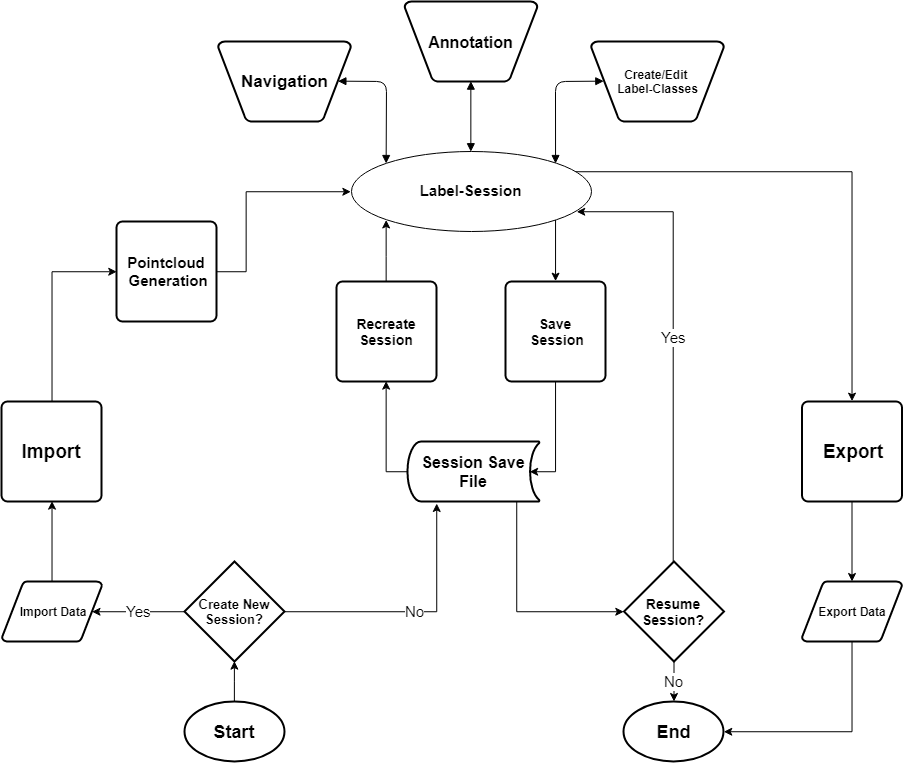
\includegraphics[width=10cm]{Workflow}
    \caption{Diagramm um den besten Machine Learning Algorithmus für eine \glslink{glos:PredAna}{Predictive-Analytics-Methoden} zu finden}
    \label{fig:Workflow}
\end{figure}

\section{Import und Export von Daten}
\label{sec:ImportExport}


\section{Architektur}

\subsection{HDF5-Beispiel}
\subsubsection{HDF5 Daten}
\subsubsection{Beispiel}

\section{Generierung einer Punktwolke}
\label{sec:Generierung}

\subsection{Generierung}
session
pointcloud
...

Koordinatensysteme

\subsection{Optimierung}
-generell nichts teures in update mehthode
	
-gameobject find
-getcomponent

keine update oder start mehtode bei skripten der punkte
collider trigger nicht bei den punkten sondern beim anderen object
generell alle pollenden aktionen von den punkten entfernen


(-clonen von prefabs statt neue instanzen von inbuilts)
shared materials verwenden   kein material.color weil das eine kopie des materials erzeugt, welches dann einzeln gecallt werden muss

gpu instancing bei den materials verwenden und forward rendering options

\section{Navigation}
\label{sec:Navigation}
\subsection{VR-Krankheit}
\subsection{Freier Flug}
\subsection{Teleport}

\section{Annotieren der Punktwolke}
\label{sec:Annotation}
\subsection{Pointer Labeling}
\subsection{Clustering}
\subsubsection{ground plane fitting}
%https://en.wikipedia.org/wiki/Singular-value_decomposition
%https://www.ltu.se/cms_fs/1.51590!/svd-fitting.pdf

\section{Ingame Menu}
\label{sec:UIMenu}
\subsection{Movement}
\subsection{Labelclasses}


